\section{Highway Networks}
Kendinden önceki yapay sinir ağlarından çok daha derin olup ilk çalışan ileri beslemeli (feed forward) sinir ağıdır. LSTM'den esinlenerek, geçiş mekanizmaları eklenmiştir. ResNet gibi ağların öncüsü olarak kabul edilir. 2015 yılındaki ImageNet yarışmasında geçişsiz bir Highway Network kullanılarak ResNet oluşturulmuştur. Kaybolan gradyanlar problemini çözmek için tasarlanmıştır. Highway Networks,  yapay sinir ağlarına ek olarak geçiş kapıları (gating mechanisms) adı verilen yapıları kullanır. Bu kapılar:
\begin{itemize}
	\item \textbf{Dönüşüm Kapısı (Transformation Gate -T)}: Hesaplanan çıktı.
	\item \textbf{Taşıma Kapısı (Carry Gate - C)}: Giriş verilerini bir sonraki katmana aktaran kapı.
	\item \textbf{Giriş Katmanı (Input Layer - x)}: Giriş verileri bu katmandan alınır.
\end{itemize}

Her katmanın çıktısı şu şekilde hesaplanır:
\[ \text{y} = H(x, W_H) * T (x, W_T) + x * C(x, W_C) \]

\begin{itemize}
	\item $H(x, W_H)$: Katman içindeki dönüşüm fonksiyonu.
	\item $T(x, W_T)$: Dönüşüm kapısı, sigmoid fonksiyonu ile elde edilen değerler.
	\item $C(x, W_C)$: Taşıma kapısı, genellikle $C(x, W_C)  = 1- T(x, W_T)$ olarak tanımlanır.
\end{itemize}

\begin{figure}[h]
    \centering
    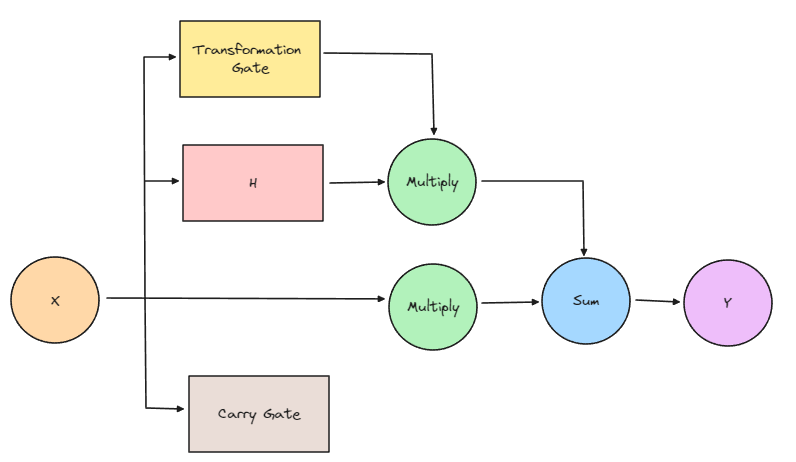
\includegraphics[width=0.7\textwidth]{images/highway_networks.png}
    \caption{Highway Networks.}
    \label{fig:enter-label}
\end{figure}

\newpage